In this chapter, we will not be discussing the results, but rather present them. This discussion will take place in Chapter 6. The results are grouped into three sections that correspond to the three main questions asked in this study. Before presenting them, we impel the reader to view Figures \ref{fig:naopostitivemap}, \ref{fig:naoneutralmapo} and \ref{fig:naonegativemapenter-label}. In addition to information about windstorm energy during different NAO phases, they illustrate the arrangement of the data points used to prepare the rest of the study. It is notable that all datapoints are positioned along the shoreline. This is an indicator that in the ERA5-Land reanalysis data, during a windstorm event, no points over the mainland exceed an hourly wind speed of 20m/s. The uncertainty introduced by this and what steps can be taken to mitigate this issue are discussed in Chapter 6.

The figures themselves are representative of all windstorms in the dataset and are divided into categories corresponding to the NAO index associated with the start of the event: NAO positive ($0.5 < \text{NAO}$), NAO neutral ($-0.5 \leq \text{NAO} \leq 0.5$) and NAO negative ($\text{NAO} < -0.5$). Figure \ref{fig:naopostitivemap} which corresponds to positive NAO events, shows considerably higher energies. Less apparent when comparing the figures with each other is the trajectory of windstorms during each NAO state. Regardless of the NAO state, high energy is always concentrated around the UK coastline; however, for NAO(+) events, energies are concentrated going North-East toward the Nordic countries through Denmark. NAO(0) events draw a trajectory that also passes through Denmark but is in the direction of Lithuania, Latvia, and Estonia. NAO(-) events take the southernmost trajectory passing through the Netherlands, Germany, Poland and towards the Ukraine. The author found that this trend can be seen most clearly when the three figures are saved and quickly flicked through back and forth to simulate a moving image. 

    \begin{figure}
        \centering
        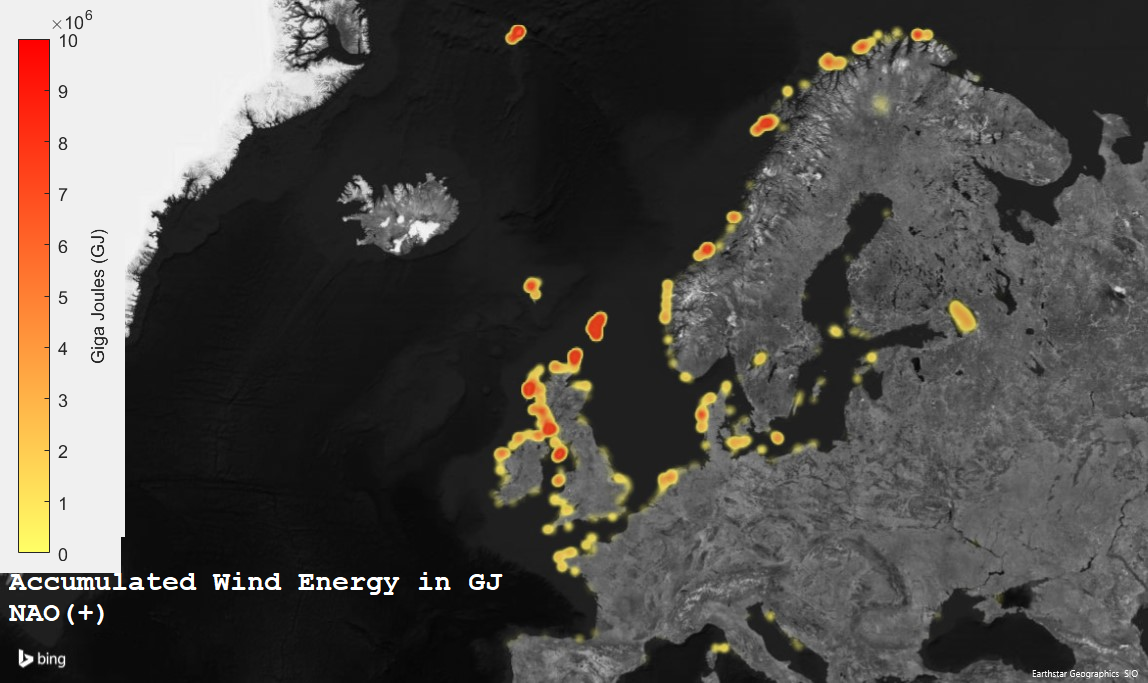
\includegraphics[width=\textwidth]{figures/NAOPOsitive.png}
        \caption{Heatmap of Energy accumulated from windstorms during NAO(+).}
        \label{fig:naopostitivemap}
    \end{figure}

    \begin{figure}
        \centering
        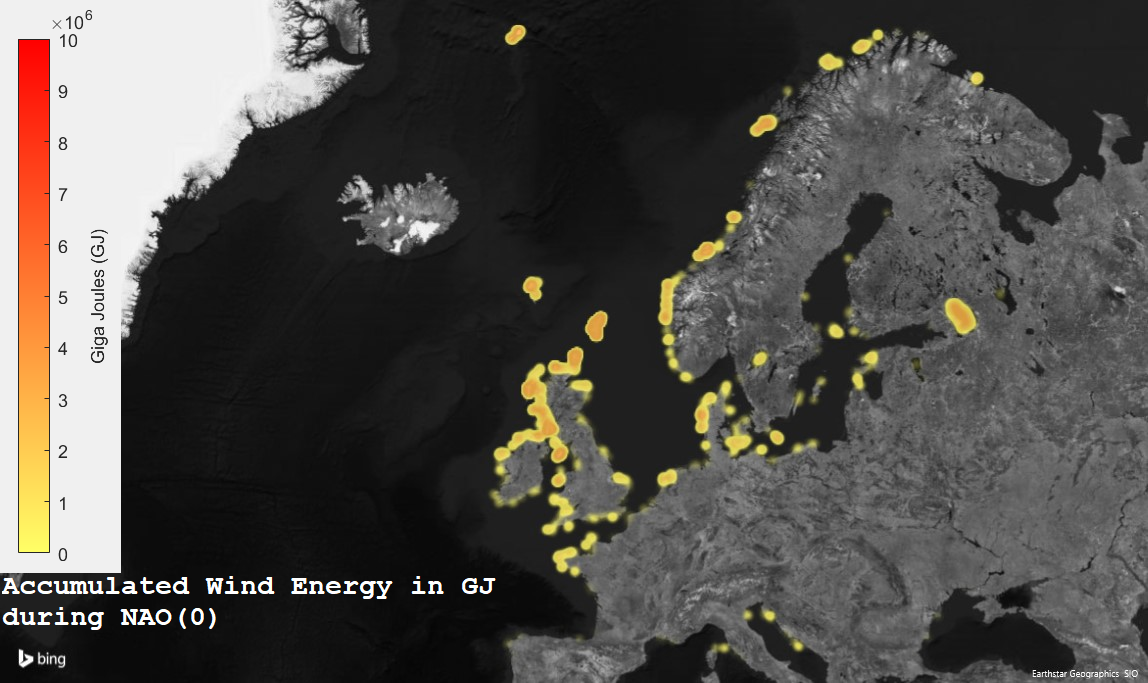
\includegraphics[width=\textwidth]{figures/NAONeutral.png}
        \caption{Heatmap of Energy accumulated from windstorms during NAO(0).}
        \label{fig:naoneutralmapo}
    \end{figure}

    \begin{figure}
        \centering
        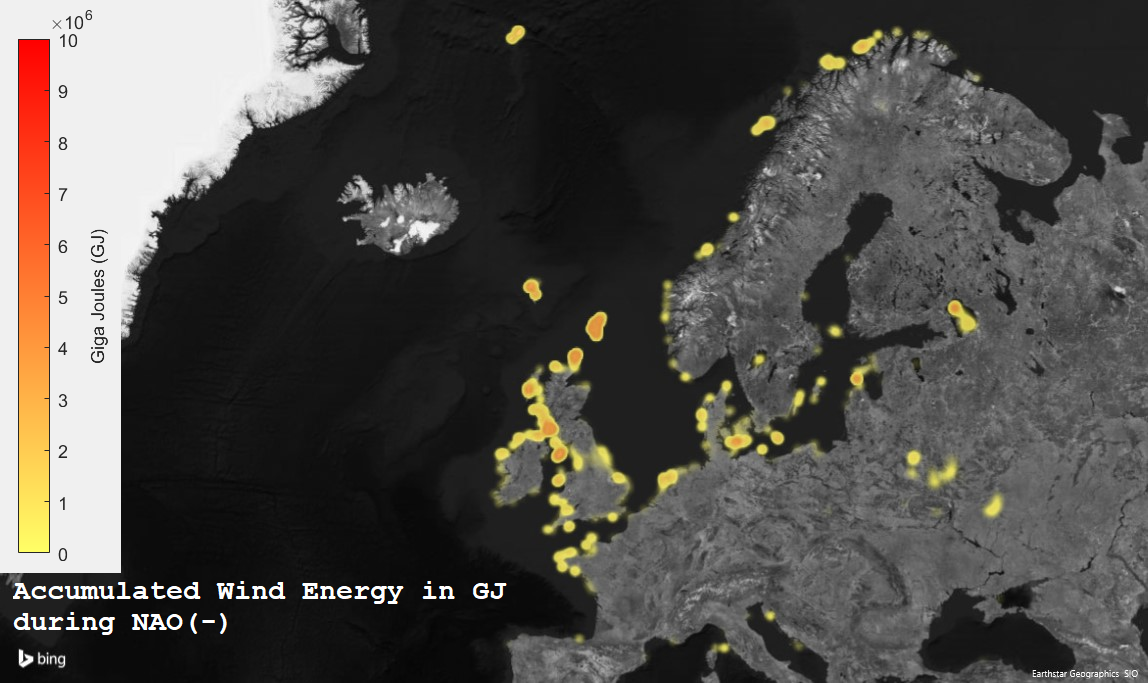
\includegraphics[width=\textwidth]{figures/NAONegative.png}
        \caption{Heatmap of Energy accumulated from windstorms during NAO(-).}
        \label{fig:naonegativemapenter-label}
    \end{figure}



\FloatBarrier
\section{Risk of European Windstorm during NAO Neutral Index}

    To estimate the return period of European Windstorms for neutral NAO phases, we will look at the statistical distribution of events and their associated indices. We begin with Figures \ref{fig:storm_count_vs_daily_nao} and \ref{fig:storm_count_vs_monthly_nao}. The former represents daily NAO values, while the latter uses monthly, where the NAO index of a windstorm is that of the first day of the event. In both cases we can see that the maximum number of events occur when the NAO is slightly positive, which agrees with the findings of \cite{https://doi.org/10.1002/joc.1982} and \cite{https://doi.org/10.1002/2014GL059647}. 

        % FIGURE 1 ------------------------------------------------------------------------------------------------------------------------
        \begin{figure}[ht]
            \begin{minipage}[t]{0.6\textwidth}
                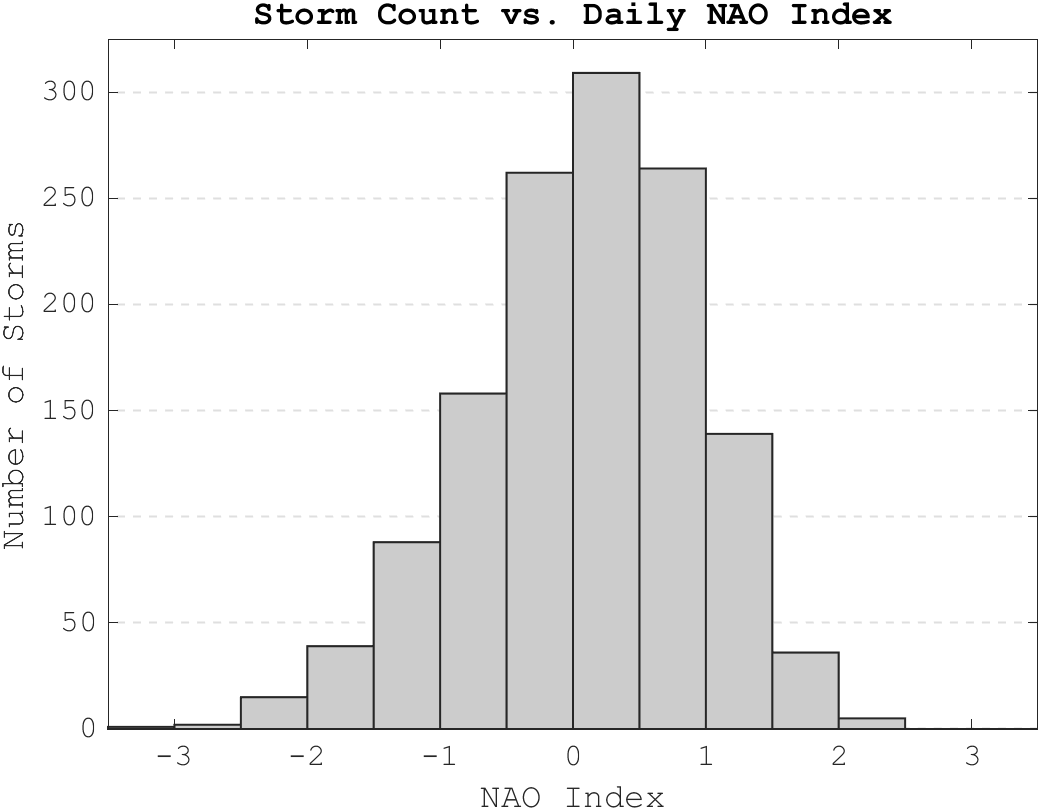
\includegraphics[width=\textwidth]{figures/Storm Count vs. Daily NAO.png}
                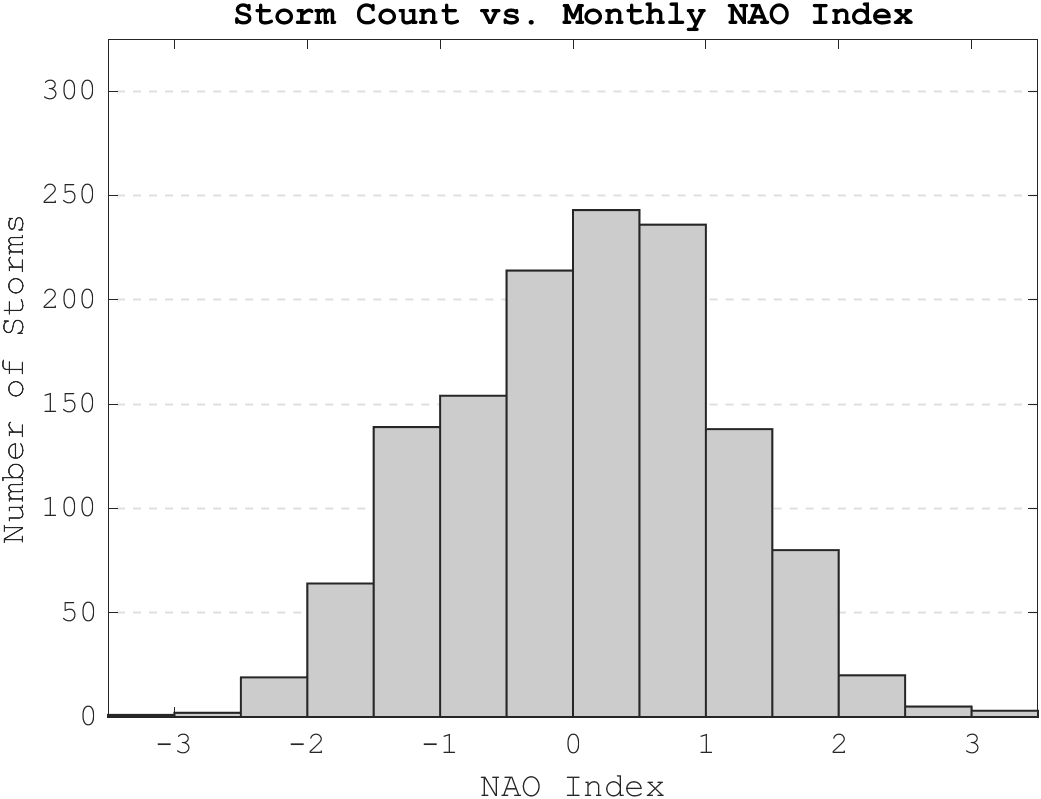
\includegraphics[width=\textwidth]{figures/Storm Count vs. Monthly NAO.png}
            \end{minipage}
            \hfill  % Fill horizontal space
            \begin{minipage}[t]{0.4\textwidth}
                \vspace*{-215pt}  % Move the start of the caption upwards. You might need to adjust this value.
                \caption{Storm Count vs. Daily NAO index from 1950 to 2020. For this figure, the NAO index of a storm is the index on the day the storm begins. The beginning of a storm in this study is defined as 36 hours before the centre (point of highest relative vorticity) of the storm touches land. N=1286.}
                \label{fig:storm_count_vs_daily_nao}
                \vspace*{88pt}  % Increase space between captions. You might need to adjust this value.
                \caption{Storm Count vs. Monthly NAO index from 1950 to 2020. Analogous to Figure \ref{fig:storm_count_vs_daily_nao}. N=1286.}
                \label{fig:storm_count_vs_monthly_nao}
            \end{minipage}
        \end{figure}
        %----------------------------------------------------------------------------------------------------------------------------------

    We follow up with an analysis of the distributing of NAO state over time. As in the last figure, we do this for both daily and monthly values in order to minimise any skewing of the data originating from inaccurately timing the start of a windstorm event. This distribution can be seen in Figure \ref{fig:nao_and_event_rate}A and Figure \ref{fig:nao_and_event_rate}C for daily and monthly values, respectively. Figures \ref{fig:nao_and_event_rate}B and \ref{fig:nao_and_event_rate}D are effectively the result of dividing the data in Figure \ref{fig:storm_count_vs_daily_nao} by that of Figure \ref{fig:nao_and_event_rate}A, and that of Figure \ref{fig:storm_count_vs_monthly_nao} by that of Figure \ref{fig:nao_and_event_rate} C, respectively, to obtain the monthly version of the spread. In \ref{fig:nao_and_event_rate}A and \ref{fig:nao_and_event_rate}C, we can see that the most probable state is when the NAO is slightly positive. In \ref{fig:nao_and_event_rate}B and \ref{fig:nao_and_event_rate}D, the probability of a windstorm occurring is uniform across all NAO states with an exception for the far ends of the data range. The author hypothesises that this is due to the very low sample size (N $<$ 5) in that range.
    
        % FIGURE 2 + FIGURE 3 -------------------------------------------------------------------------------------------------------------
        \begin{figure}
            \centering
            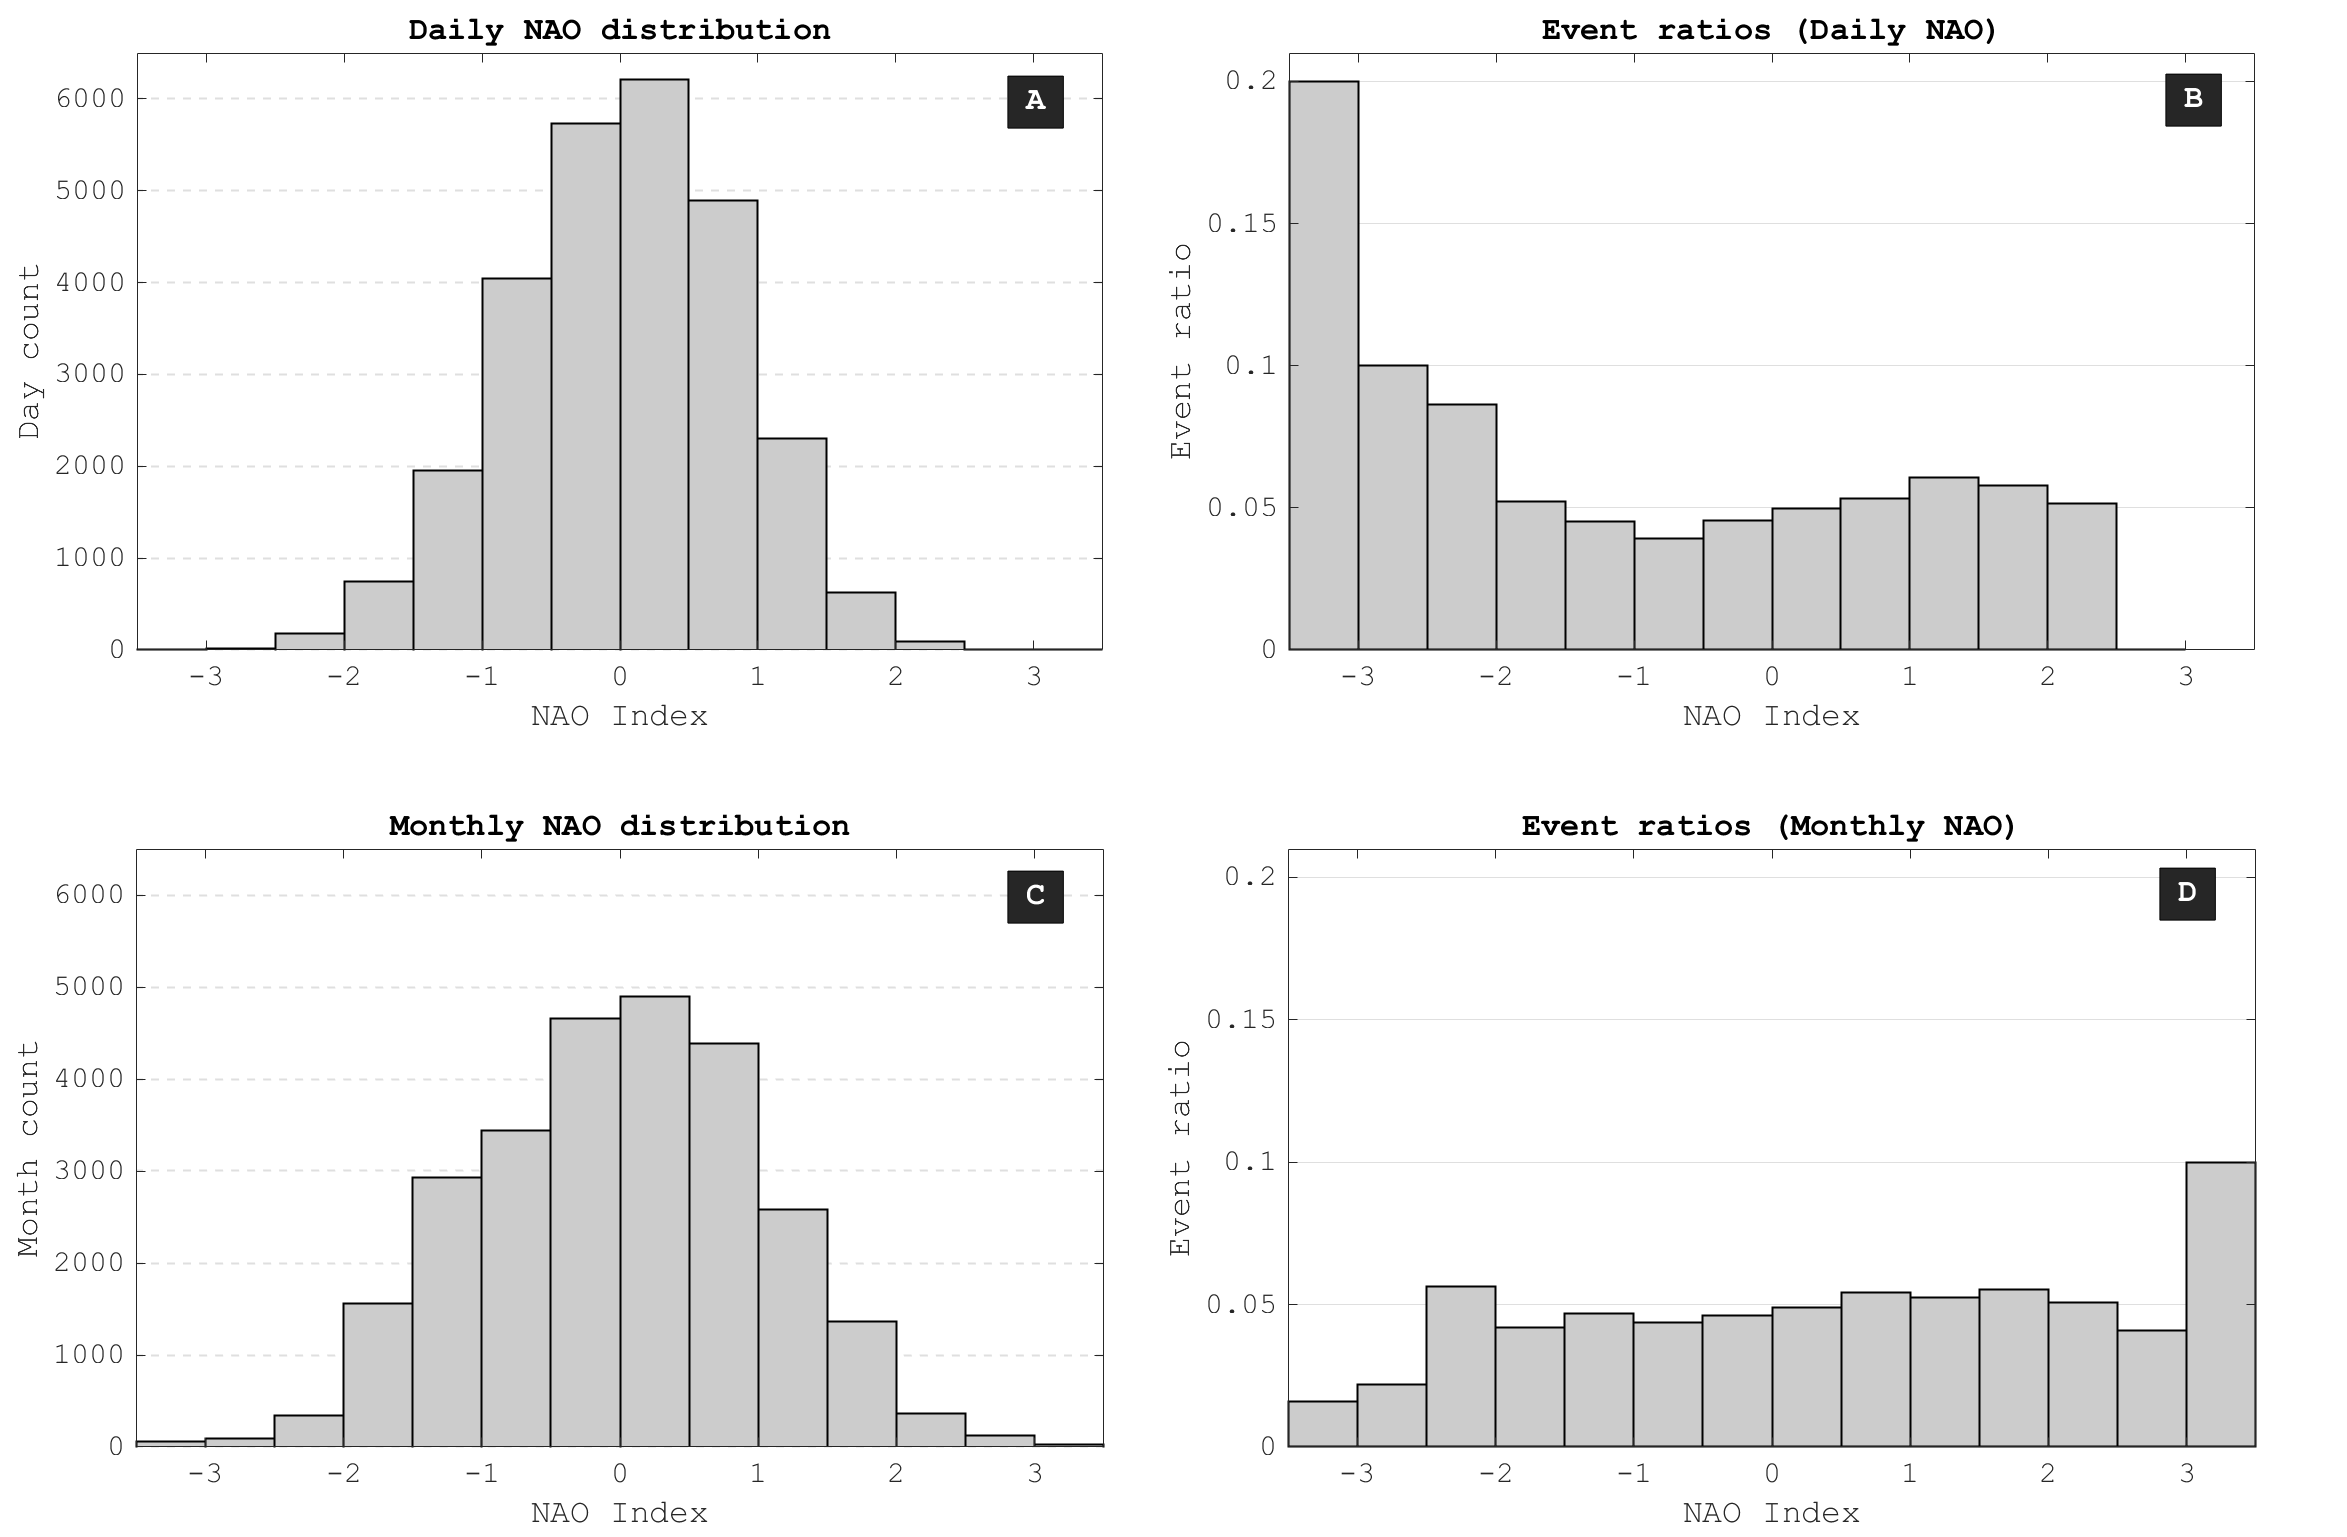
\includegraphics[width=\textwidth]{figures/nao_state_as_four_1.52.png}
            \caption{For this figure, the NAO index of a storm is the index at the day on which the storm begins. The beginning of a storm in this study is defined as 36 hours before the centre (point of highest relative vorticity) of the storm touches land. The NAO index is sourced from the NOAA archive. \textbf{A:} Daily NAO distribution. Represents the number of days that fall within a certain NAO index, starting from -3.5 to 3.5 with steps of 0.5. The peak of the graph lies in the range of 0.0 to 0.5. \textbf{C:} Monthly NAO distribution. The peak of the graph lies in the range 0.0 to 0.5. \textbf{B:} Represents the number of windstorm events associated with a NAO state divided by the total number of days that have had that NAO state. 20\% of days with a NAO index between -3.5 and -3.0 have experienced a windstorm, which is the highest event rate in this figure. The event rates for other NAO instances vary from 5\% to 10\% with no pronounced pattern. \textbf{D:} Monthly Windstorm Event Ratio. 10\% of days with a NAO index between +3.0 and +3.5 have experienced a windstorm, which is the highest event rate in this figure. Event rates for other NAO indices vary between 2\% to 6\% with no pronounced pattern.}
            \label{fig:nao_and_event_rate}
        \end{figure}
        %----------------------------------------------------------------------------------------------------------------------------------

    In Figure \ref{fig:normalized_probability_of_storm_events_with_NAO}, we present the probabalistic distribution of windstorm events by month, further broken down into NAO states. The height of all 12 columns adds up to $1.00$ and they are always stacked so that NAO(-) is on top and NAO (+) at the bottom. The months that have observed the most number of events are December, January, November and February in descending order, while the least events occurred in June, July and August in ascending order. These rates are consistent with previous papers such as those by \cite{Hurrell2003}, \cite{Renggli2011}, and others, where the winter period is associated with a high rate of windstorms, while the summer observes only occasional events. Months with a significant probability of windstorms tend to have events evenly spread between NAO(0) and NAO(-), with a slight tendency towards NAO(0). NAO(-) events are not rare but are consistently less probable than their counterparts.

        % FIGURE 5 ------------------------------------------------------------------------------------------------------------------------
        \sidecaptionvpos{figure}{t}
        \begin{SCfigure}
            \centering
            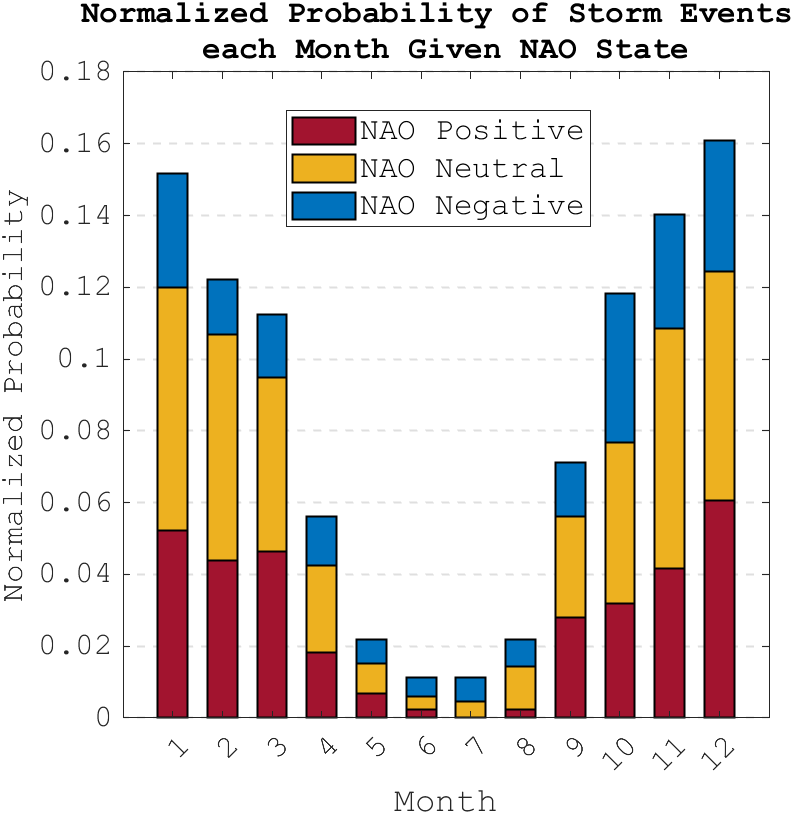
\includegraphics[width=0.6\textwidth]{figures/Normalized Probability of Storm Events Given NAO State(small).png}
            \caption{Represents the probability of observing a windstorm event during each month of the year, sectioned by the NAO index which corresponds to the beggining of the storm. NAO neutral indices are those which belong in the range of -0.5 to 0.5 including. The beginning of a storm in this study is defined as 36 hours before the centre (point of highest relative vorticity) of the storm touches land.}
            \label{fig:normalized_probability_of_storm_events_with_NAO}
        \end{SCfigure}
        %----------------------------------------------------------------------------------------------------------------------------------

    In addition to Figure \ref{fig:normalized_probability_of_storm_events_with_NAO}, we present Figure \ref{fig:averageEnergyPerMonth}. In it we present the average energy of a windstorm event for each month, once again splitting events into categories based on the NAO state they are associated with. Embed on top of each bar is the number of events that go into the respective category in the form 'N =...'. When looking at the boreal winter period of December-January-February, NAO (+) windstorms are significantly more energetic. For the remainder of the year, windstorm energy is more evenly distributed between the three NAO states, with no directly apparent pattern to which is the most energetic.

        % FIGURE 6 ------------------------------------------------------------------------------------------------------------------------
        \begin{figure}
            \centering
            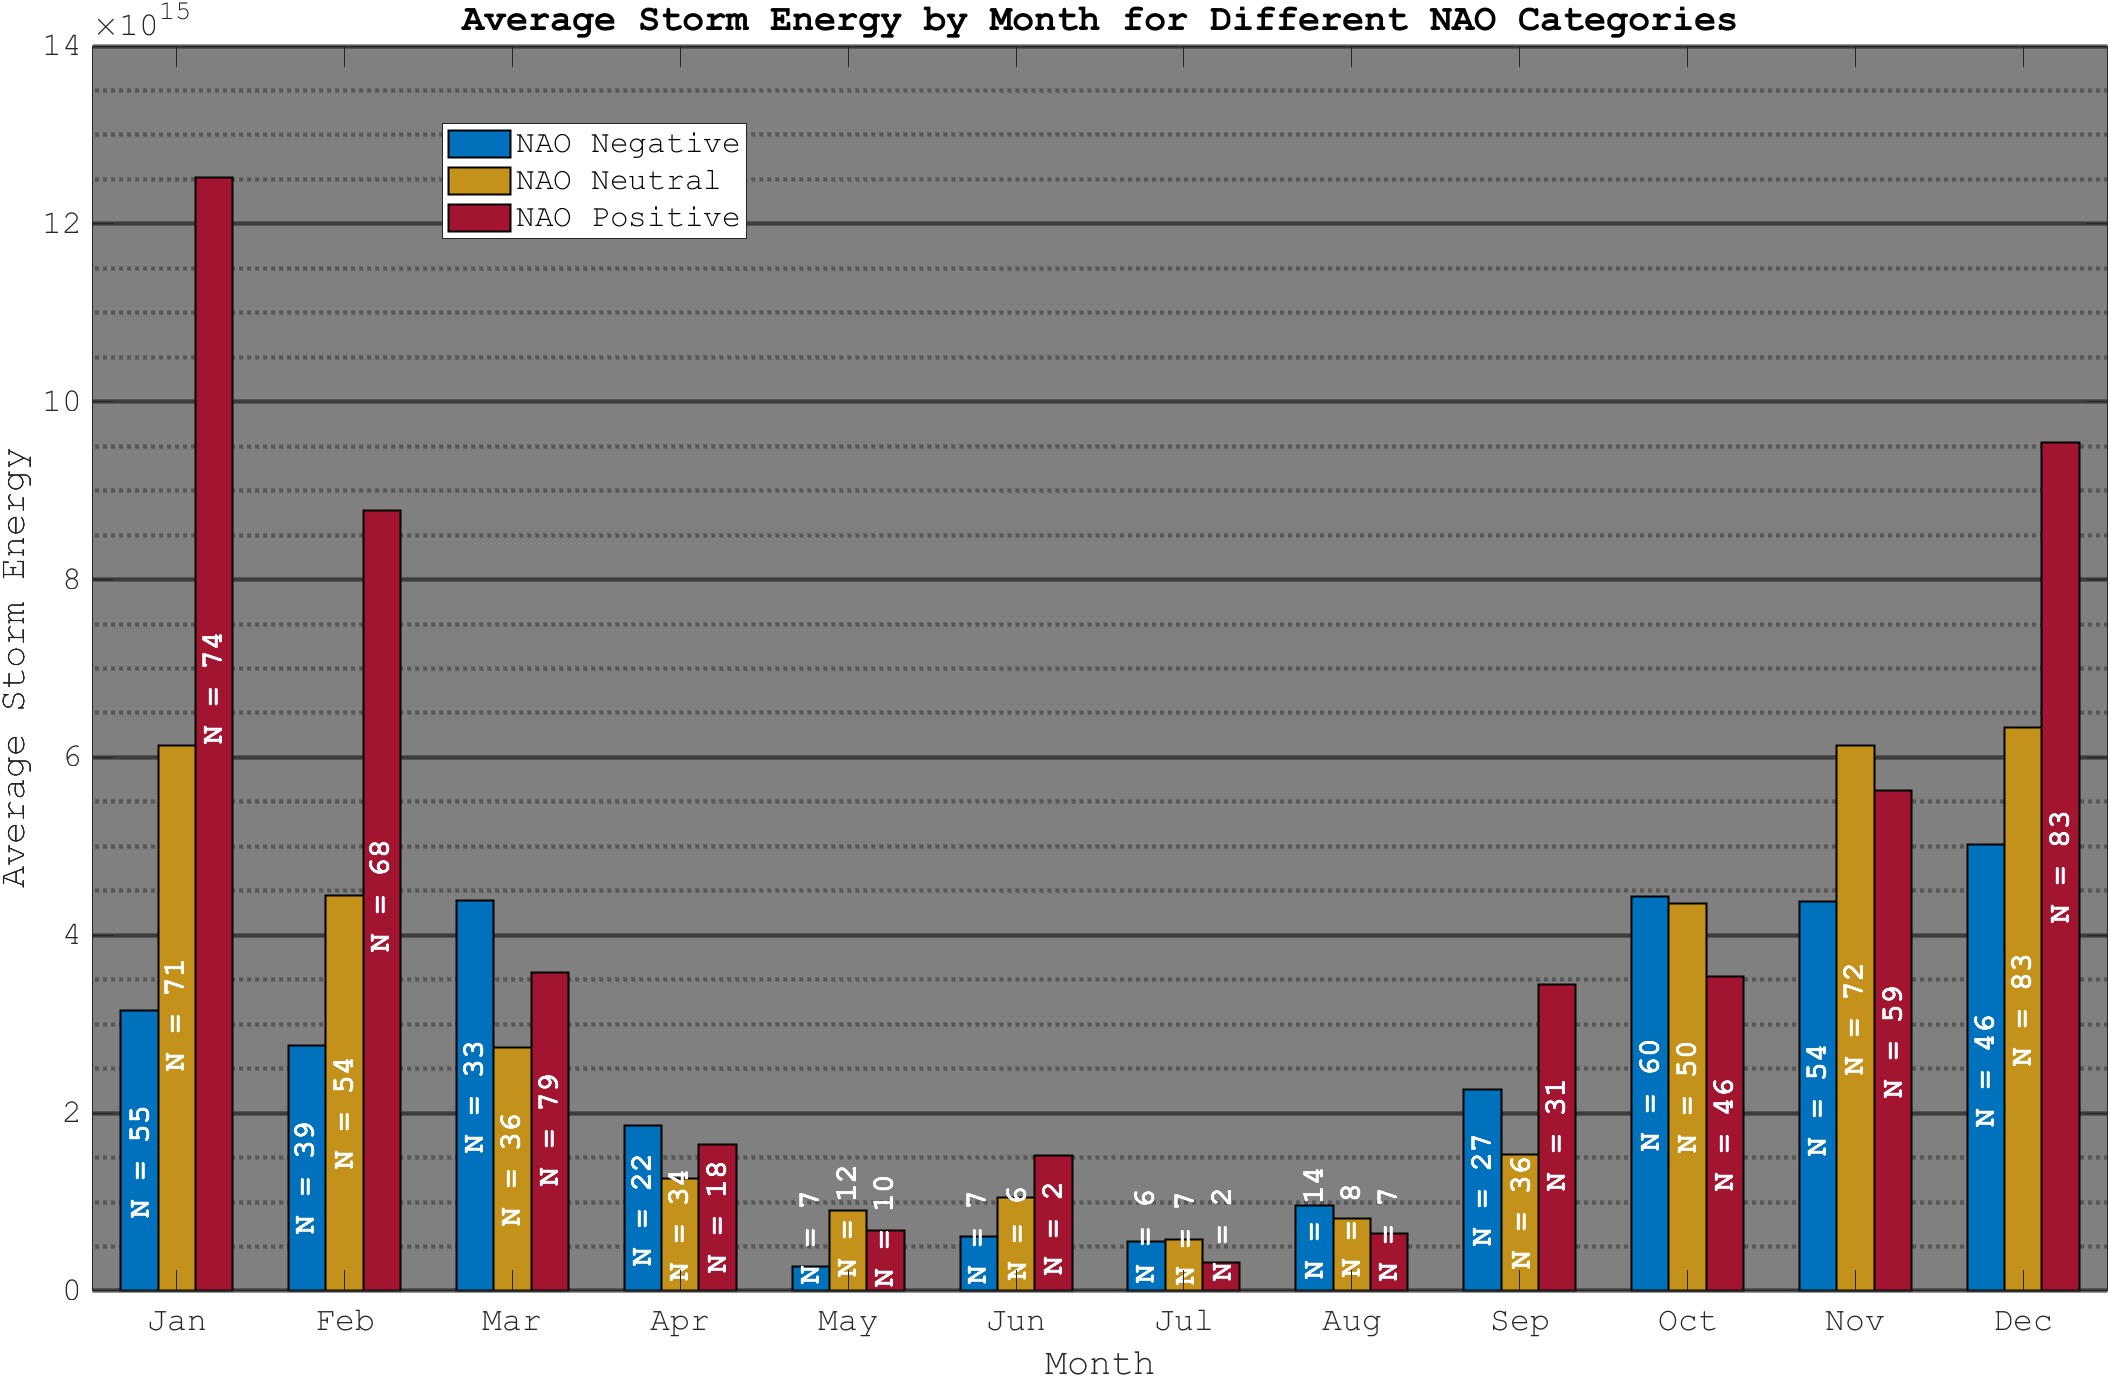
\includegraphics[width=\textwidth]{figures/average_storm_energy_by_month_with_nao_separated.png}
            \caption{Represents the probability of observing a windstorm event during each month of the year, sectioned by the NAO index which corresponds to the beggining of the storm. NAO neutral indices are those which belong in the range of -0.5 to 0.5 including. The beginning of a storm in this study is defined as 36 hours before the centre (point of highest relative vorticity) of the storm touches land.}
            \label{fig:averageEnergyPerMonth}
        \end{figure}
        %----------------------------------------------------------------------------------------------------------------------------------



\FloatBarrier
\section{The Influence of a Longer Dataset on Results}

    Studies on windstorms are limited in terms of data, and depending on the desired accuracy, this range roughly varies from 70 to 30 years. To investigate the effect that different time ranges have on the statistical relationship between windstorms and the NAO, we obtain the exceedance probability of windstorms in western Europe excluding Iceland for three different periods: one where the NAO is predominantly in a positive state, one where it is in a negative state, and one where the average state of the NAO approximates to neutral. Note that the last does not mean that the period is composed of NAO neutral years, but rather NAO negative and NAO positive states are equally represented. 

    The first step is to determine the range for each of the aforementioned periods. To do this, we take the yearly NAO state to be equal to the average of the monthly ones. We present the results in Figure \ref{fig:yearlyNAO}. From it we identify the time between 1950 to 1970 as dominated by a NAO(-) state. 1970 to 2000 is dominated by a NAO(+) state, and we estimate the period from 2000 to 2020 to be balanced.
    
        % FIGURE XTRA #1 ------------------------------------------------------------------------------------------------------------------
        \sidecaptionvpos{figure}{t}
        \begin{SCfigure}
            \centering
            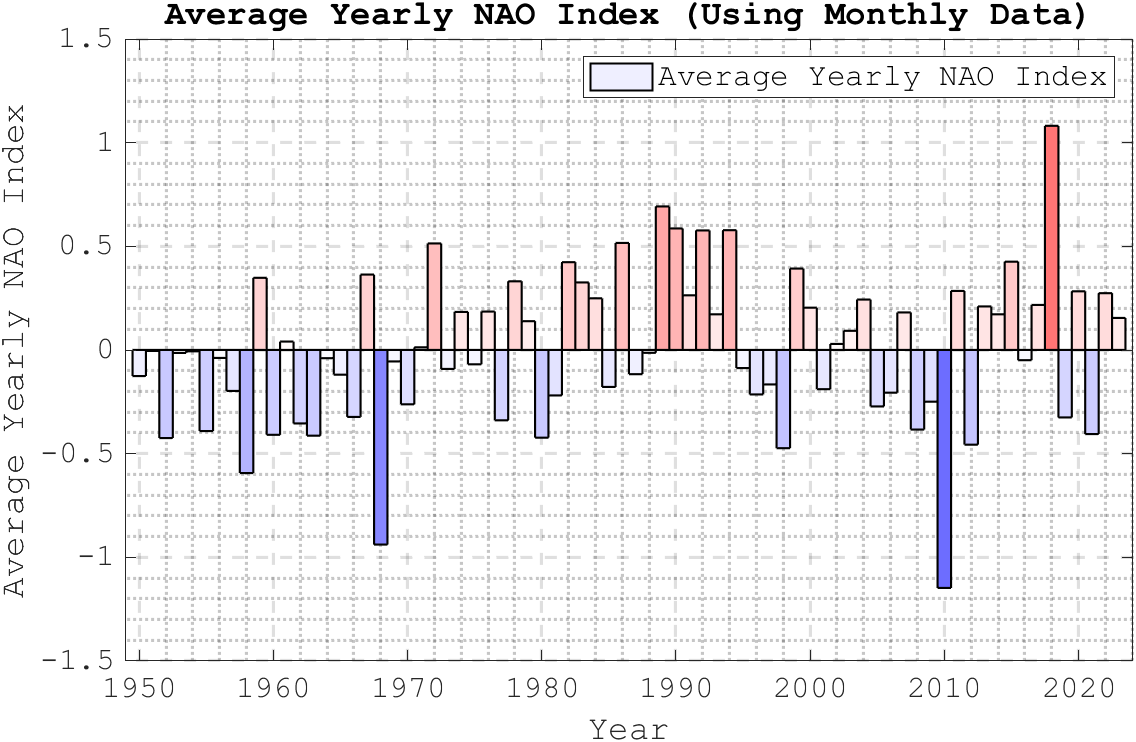
\includegraphics[width=0.7\textwidth]{figures/Average_NAO_Index_Yearly_from_month.png}
            \caption{ Each bar represents the NAO Index for that year as obtained from taking the average of the NAO monthly index.}
            \label{fig:yearlyNAO}
        \end{SCfigure}
        %----------------------------------------------------------------------------------------------------------------------------------

    We also present the EP for the entire period used in this study, beginning in 1950 and ending in 2020 in Figure \ref{fig:EP_Curve_NAO(p,n)_1950-2020}. In it we mark the position of several named storms in the data for added clarity. The figure shows a clear division between NAO(+,0,-) windstorms, with NAO(+) events being the most energetic and NAO(-) events the least energetic. Storms Kyrill and Lothar align with expectations, appearing at the curve's tail. Contrarily, Storm Klaus ranks in the top 40\% of high-energy NAO(-) events, illustrating that a storm's perceived impact isn't solely determined by its strength, but also by its trajectory, such as whether it passes over open land or populated areas.

        % FIGURE 4 ------------------------------------------------------------------------------------------------------------------------
        \sidecaptionvpos{figure}{t}
        \begin{SCfigure}
            \centering
            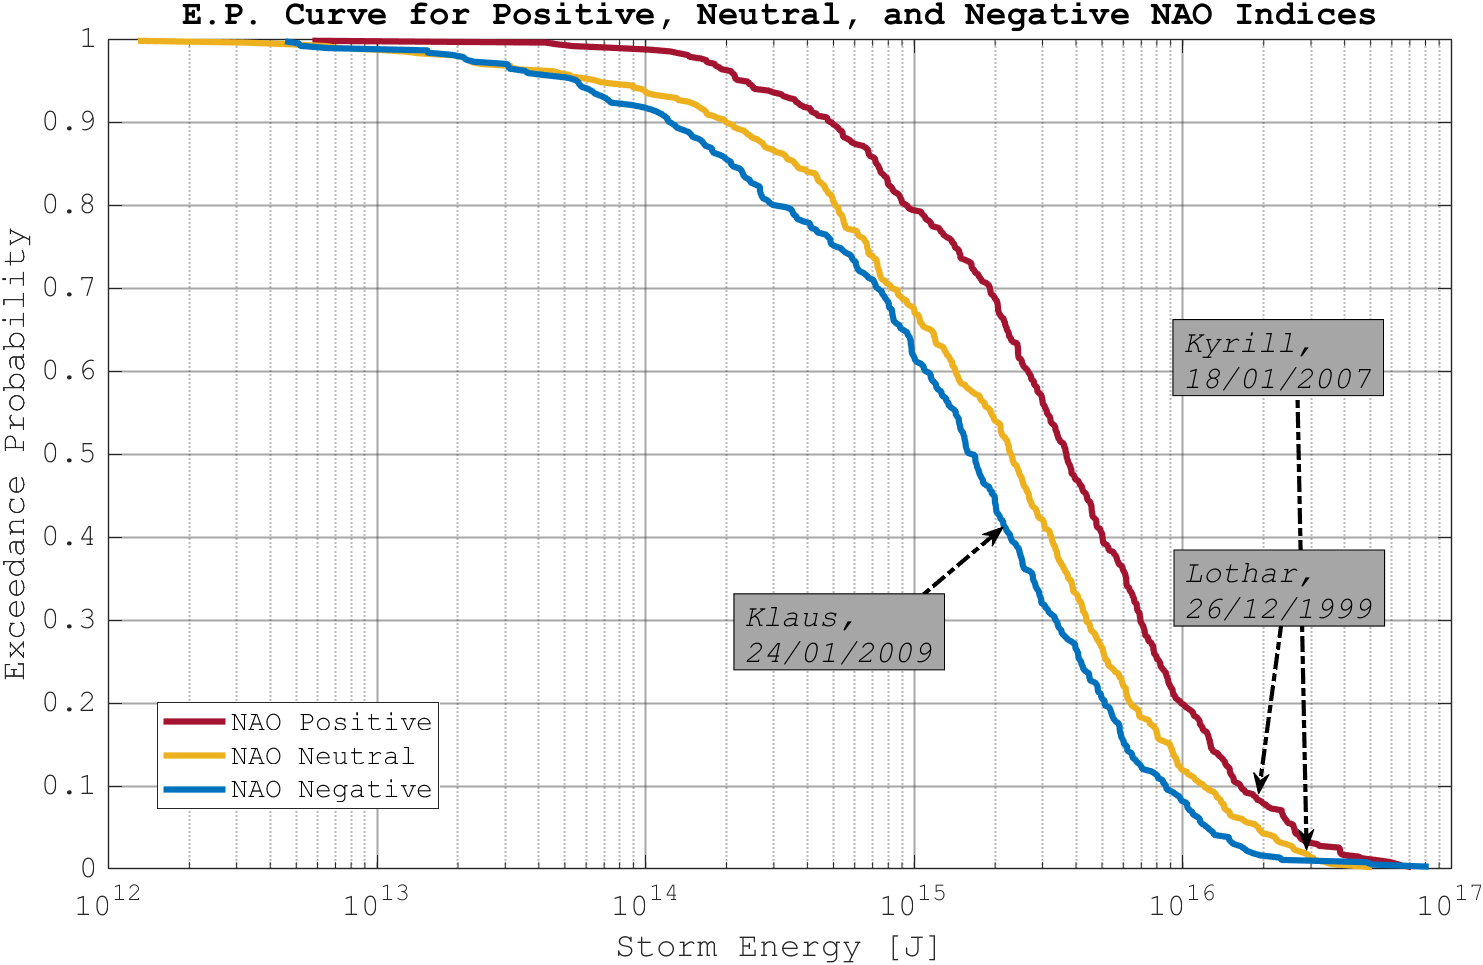
\includegraphics[width=0.7\textwidth]{figures/EP Curve NAO(p,n), 1950-2020(small)_with_neutral_nao.png}
            \caption{Exceedance probability curve for positive, negative and neutral NAO. Data are obtained from windstorm energy estimations as presented in this study and the NOAA NAO index database for the period of 1950 to 2020. The position of some named storms is shown for perspective.}
            \label{fig:EP_Curve_NAO(p,n)_1950-2020}
        \end{SCfigure}
        %----------------------------------------------------------------------------------------------------------------------------------

        % TABLE 1 -------------------------------------------------------------------------------------------------------------------------
        \begin{table}
        \centering
        \resizebox{\textwidth}{!}{%
        \begin{tabular}{ccccccccccc}
         &
          \multicolumn{1}{c|}{} &
          \multicolumn{3}{c|}{\textbf{N}} &
          \multicolumn{3}{c|}{\textbf{Mean Energy {[}$10^{15}$J{]}}} &
          \multicolumn{3}{c}{\textbf{Median Energy {[}$10^{15}$J{]}}} \\
         &
          \multicolumn{1}{c|}{D.S.} &
          \cellcolor[HTML]{FFCCC9}\textbf{NAO(+)} &
          \cellcolor[HTML]{FFFFC7}\textbf{NAO(0)} &
          \multicolumn{1}{c|}{\cellcolor[HTML]{ECF4FF}\textbf{NAO(-)}} &
          \cellcolor[HTML]{FFCCC9}\textbf{NAO(+)} &
          \cellcolor[HTML]{FFFFC7}\textbf{NAO(0)} &
          \multicolumn{1}{c|}{\cellcolor[HTML]{ECF4FF}\textbf{NAO(-)}} &
          \cellcolor[HTML]{FFCCC9}\textbf{NAO(+)} &
          \cellcolor[HTML]{FFFFC7}\textbf{NAO(0)} &
          \cellcolor[HTML]{ECF4FF}\textbf{NAO(-)} \\
        {\color[HTML]{00009B} 1950:1970} &
          \multicolumn{1}{c|}{{\color[HTML]{00009B} -'ve}} &
          \cellcolor[HTML]{FFCCC9}{\color[HTML]{00009B} 98} &
          \cellcolor[HTML]{FFFFC7}{\color[HTML]{00009B} 126} &
          \multicolumn{1}{c|}{\cellcolor[HTML]{ECF4FF}{\color[HTML]{00009B} 150}} &
          \cellcolor[HTML]{FFCCC9}{\color[HTML]{00009B} 5.2} &
          \cellcolor[HTML]{FFFFC7}{\color[HTML]{00009B} 5.2} &
          \multicolumn{1}{c|}{\cellcolor[HTML]{ECF4FF}{\color[HTML]{00009B} 3.7}} &
          \cellcolor[HTML]{FFCCC9}{\color[HTML]{00009B} 2.8} &
          \cellcolor[HTML]{FFFFC7}{\color[HTML]{00009B} 2.8} &
          \cellcolor[HTML]{ECF4FF}{\color[HTML]{00009B} 1.5} \\
        {\color[HTML]{680100} 1970:2000} &
          \multicolumn{1}{c|}{{\color[HTML]{680100} +'ve}} &
          \cellcolor[HTML]{FFCCC9}{\color[HTML]{680100} 224} &
          \cellcolor[HTML]{FFFFC7}{\color[HTML]{680100} 207} &
          \multicolumn{1}{c|}{\cellcolor[HTML]{ECF4FF}{\color[HTML]{680100} 152}} &
          \cellcolor[HTML]{FFCCC9}{\color[HTML]{680100} 7.5} &
          \cellcolor[HTML]{FFFFC7}{\color[HTML]{680100} 4.4} &
          \multicolumn{1}{c|}{\cellcolor[HTML]{ECF4FF}{\color[HTML]{680100} 3.8}} &
          \cellcolor[HTML]{FFCCC9}{\color[HTML]{680100} 3.8} &
          \cellcolor[HTML]{FFFFC7}{\color[HTML]{680100} 2.2} &
          \cellcolor[HTML]{ECF4FF}{\color[HTML]{680100} 2.0} \\
        {\color[HTML]{656565} 2000:2020} &
          \multicolumn{1}{c|}{{\color[HTML]{656565} -/-}} &
          \cellcolor[HTML]{FFCCC9}{\color[HTML]{656565} 153} &
          \cellcolor[HTML]{FFFFC7}{\color[HTML]{656565} 133} &
          \multicolumn{1}{c|}{\cellcolor[HTML]{ECF4FF}{\color[HTML]{656565} 82}} &
          \cellcolor[HTML]{FFCCC9}{\color[HTML]{656565} 7.1} &
          \cellcolor[HTML]{FFFFC7}{\color[HTML]{656565} 4.3} &
          \multicolumn{1}{c|}{\cellcolor[HTML]{ECF4FF}{\color[HTML]{656565} 2.5}} &
          \cellcolor[HTML]{FFCCC9}{\color[HTML]{656565} 3.8} &
          \cellcolor[HTML]{FFFFC7}{\color[HTML]{656565} 2.2} &
          \cellcolor[HTML]{ECF4FF}{\color[HTML]{656565} 1.0} \\ \hline
        1950:2020 &
           &
          \cellcolor[HTML]{FFCCC9}465 &
          \cellcolor[HTML]{FFFFC7}462 &
          \cellcolor[HTML]{ECF4FF}364 &
          \cellcolor[HTML]{FFCCC9}6.9 &
          \cellcolor[HTML]{FFFFC7}4.6 &
          \cellcolor[HTML]{ECF4FF}3.5 &
          \cellcolor[HTML]{FFCCC9}3.7 &
          \cellcolor[HTML]{FFFFC7}2.3 &
          \cellcolor[HTML]{ECF4FF}1.6
        \end{tabular}%
        }
        \caption{Table with statistical information about Figures \ref{fig:EP19501970}, \ref{fig:EP19702000}, \ref{fig:EP20002020} and \ref{fig:EP_Curve_NAO(p,n)_1950-2020}. Dominant state for period given in D.S. column}
        \label{tab:eptable}
        \end{table}
        %----------------------------------------------------------------------------------------------------------------------------------

    In Figures \ref{fig:EP19501970}, \ref{fig:EP19702000} and \ref{fig:EP20002020} we present the EP curves for the earlier defined periods. Statistics such as the number of members, mean and median energy can be found in Table \ref{tab:eptable}. 

        % FIGURE 12 -----------------------------------------------------------------------------------------------------------------------
        \begin{figure}[ht]
            \begin{minipage}[t]{0.7\textwidth}
                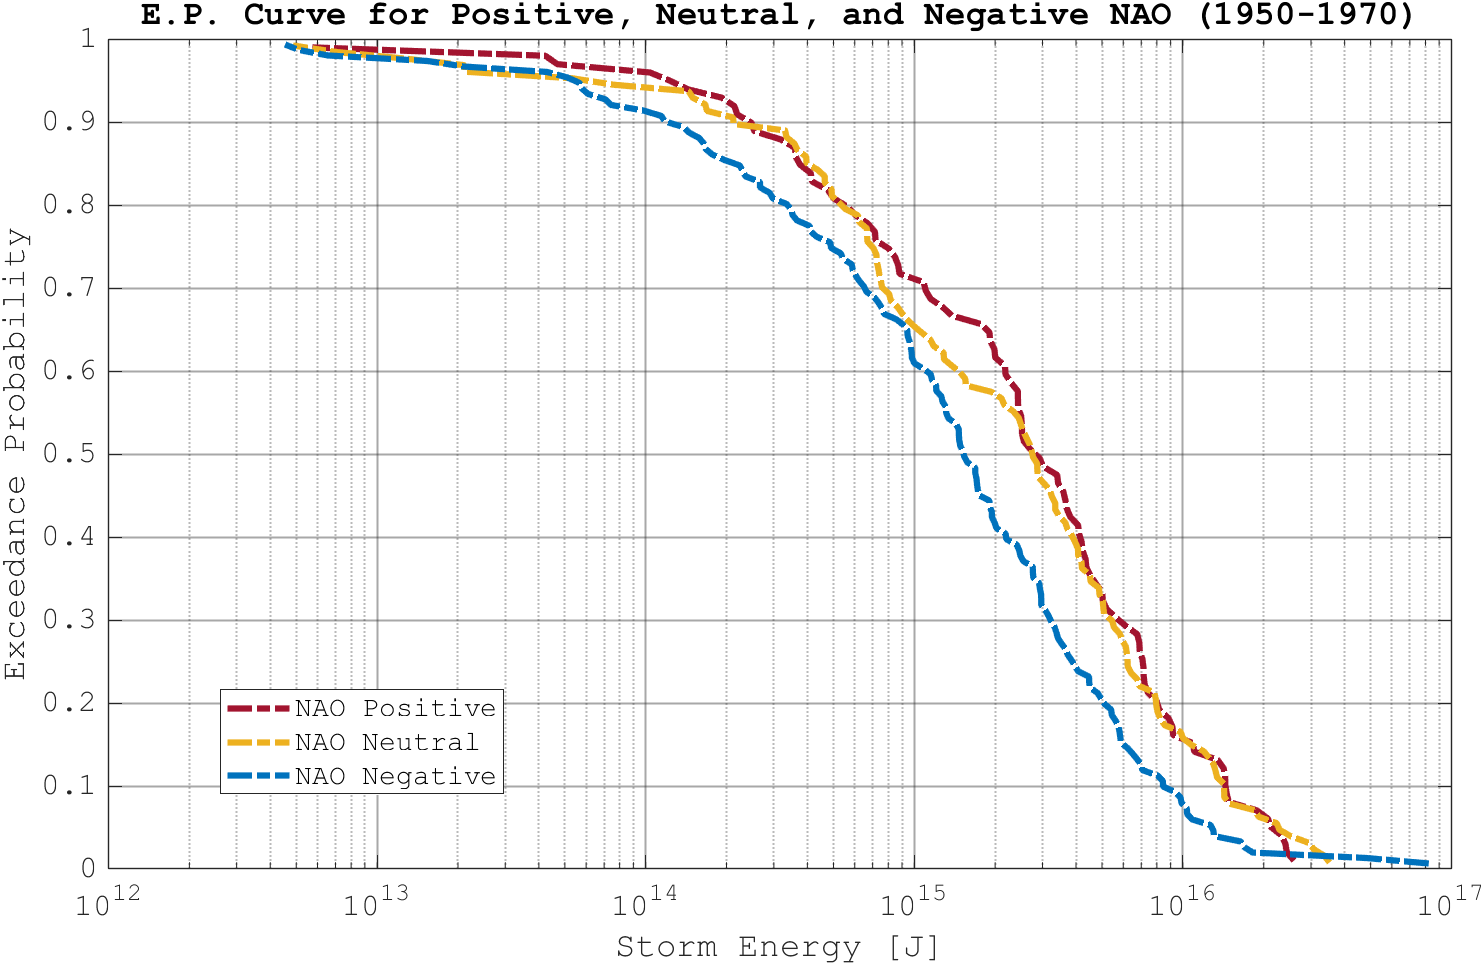
\includegraphics[width=\textwidth]{figures/EP_curve_1950_1970.png}
                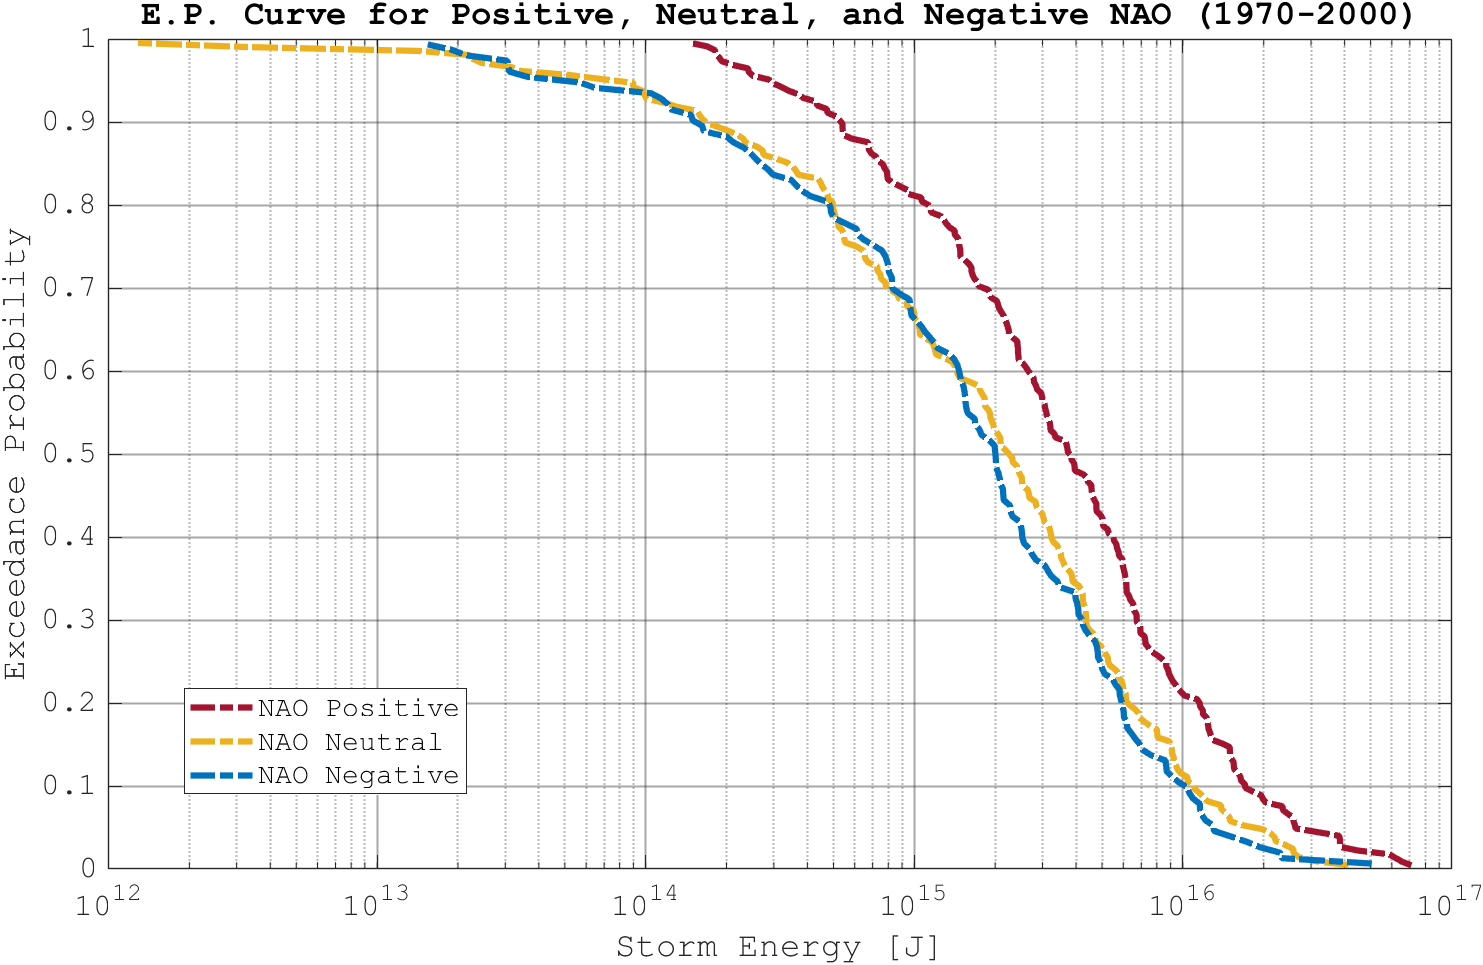
\includegraphics[width=\textwidth]{figures/EP_curve_1970_2000.png}
                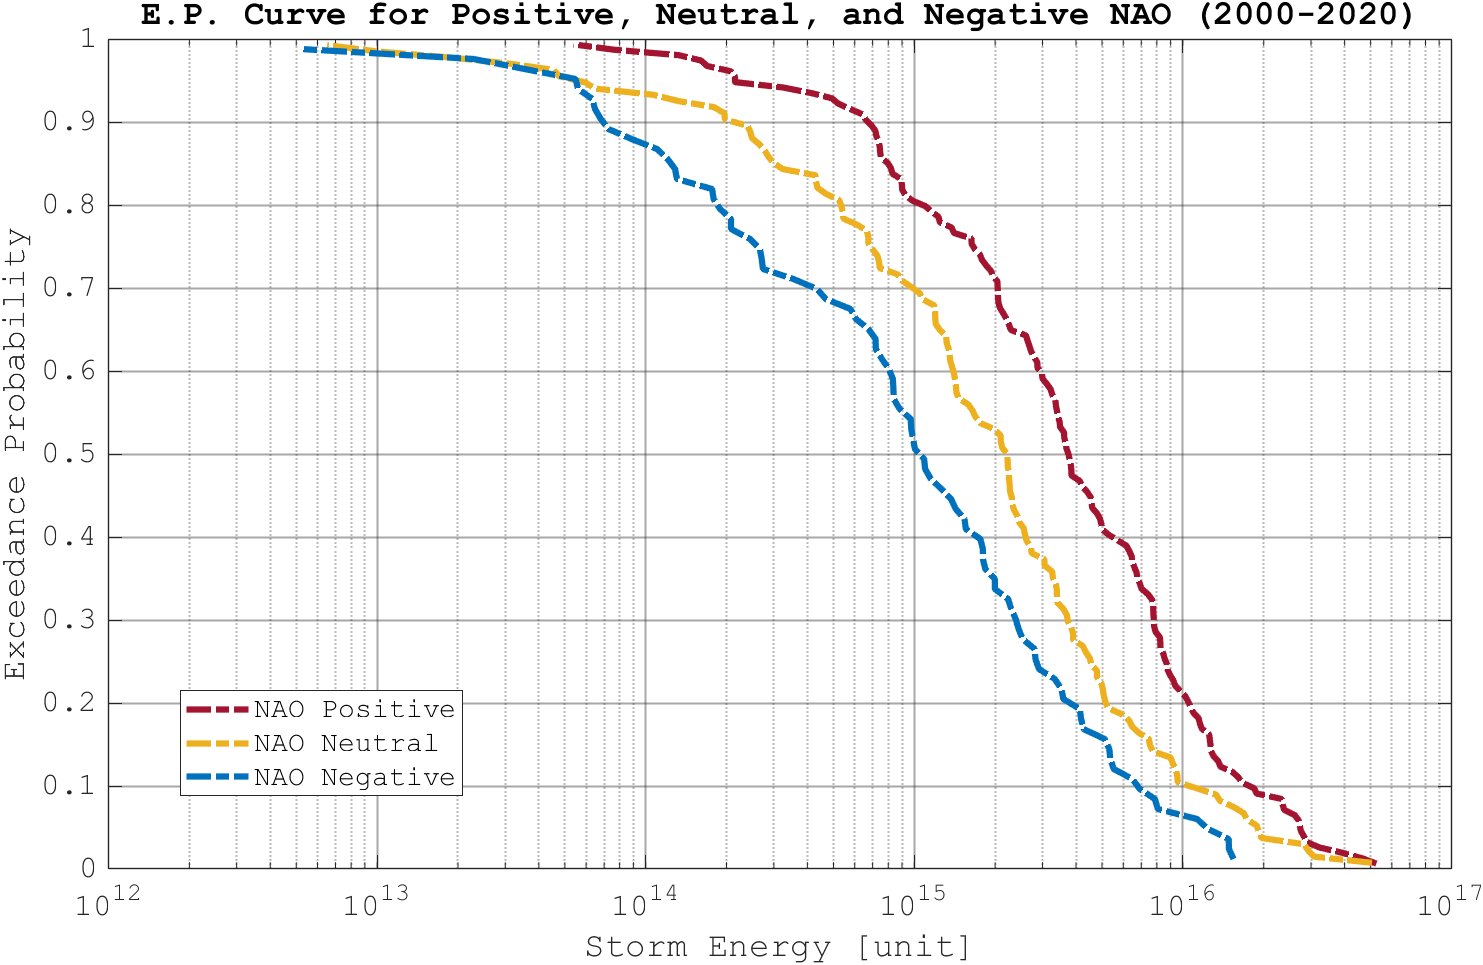
\includegraphics[width=\textwidth]{figures/EP_curve_2000_2020.png}
            \end{minipage}
            \hfill  % Fill horizontal space
            \begin{minipage}[t]{0.29\textwidth}
                \vspace*{-215pt}  % Move the start of the caption upwards. You might need to adjust this value.
                \caption{Exceedance probability curve for positive, negative and neutral NAO for the period 1950 to 1970. Mean Energy in PetaJoules: NAO(+)~5.2, NAO(0)~5.2, NAO(-)~3.7}
                \label{fig:EP19501970}
                \vspace*{110pt}  % Increase space between captions. You might need to adjust this value.
                \caption{Exceedance probability curve for positive, negative and neutral NAO for the period 1970 to 2000. Mean Energy in PetaJoules: NAO(+)~7.5, NAO(0)~4.4, NAO(-)~3.8}
                \label{fig:EP19702000}
                \vspace*{110pt}  % Increase space between captions. You might need to adjust this value.
                \caption{Exceedance probability curve for positive, negative and neutral NAO for the period 2000 to 2020. Mean Energy in PetaJoules: NAO(+)~7.1, NAO(0)~4.3, NAO(-)~2.5}
                \label{fig:EP20002020}
            \end{minipage}
        \end{figure}
        %----------------------------------------------------------------------------------------------------------------------------------

\FloatBarrier
\section{The Influence of the NAO State on Windstorm Paths in Europe}

    To investigate the path taken by storms during different states of the NAO we produce two sets of figures. In one we present the distribution of energy from our windstorm dataset divided into the country over which the energy was released. The set contains this for two time periods - boreal winter and boreal summer given in Figures \ref{fig:DJF_Tot_Eng_by_cunt} and \ref{fig:JJA_Tot_Eng_by_cunt}, respectively. Note that the energy during boreal summer is two orders of magnitude lower than that during boreal winter. During the December to January period windstorm energy is concentrated in the UK, Spain, Belgium, and Norway, in that order. During the June to August period, windstorm energy is highest in the UK, Denmark, Norway, and Belgium.
    
        % FIGURE 7 + 8 --------------------------------------------------------------------------------------------------------------------
        \begin{figure}[ht]
            \begin{minipage}[t]{0.59\textwidth}
                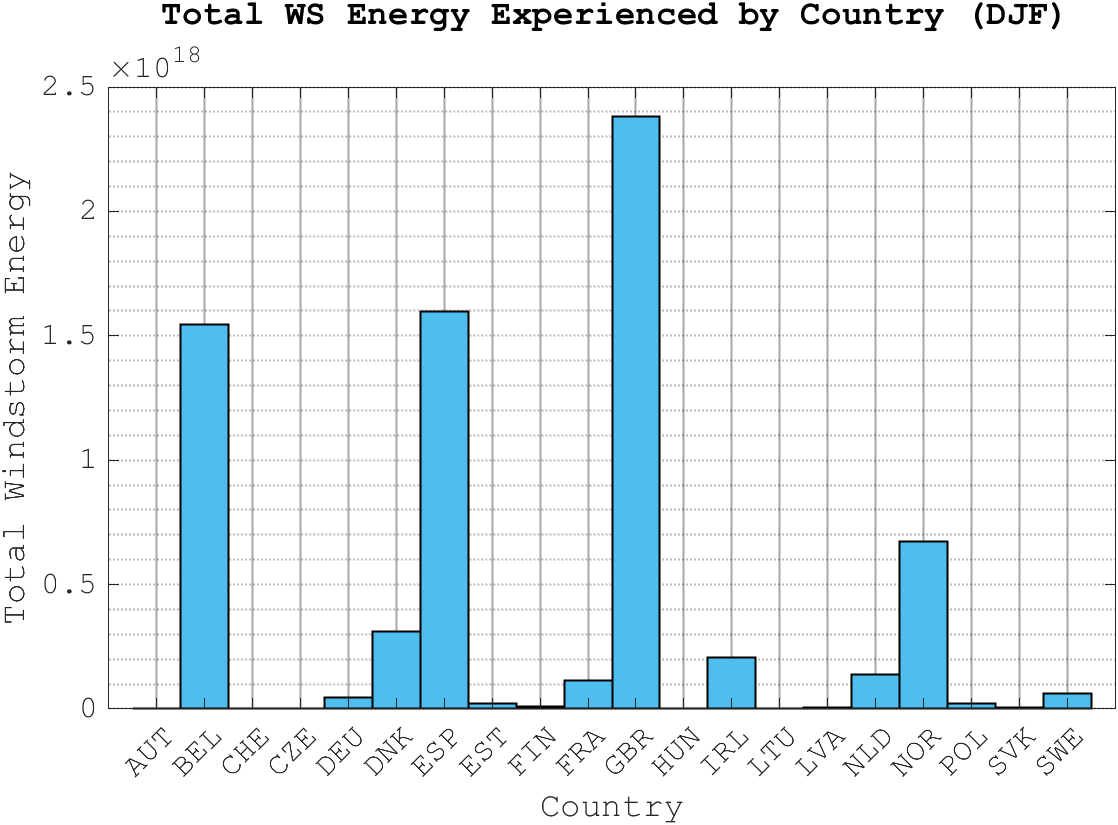
\includegraphics[width=\textwidth]{figures/Total Energy of WS DJF.png}
                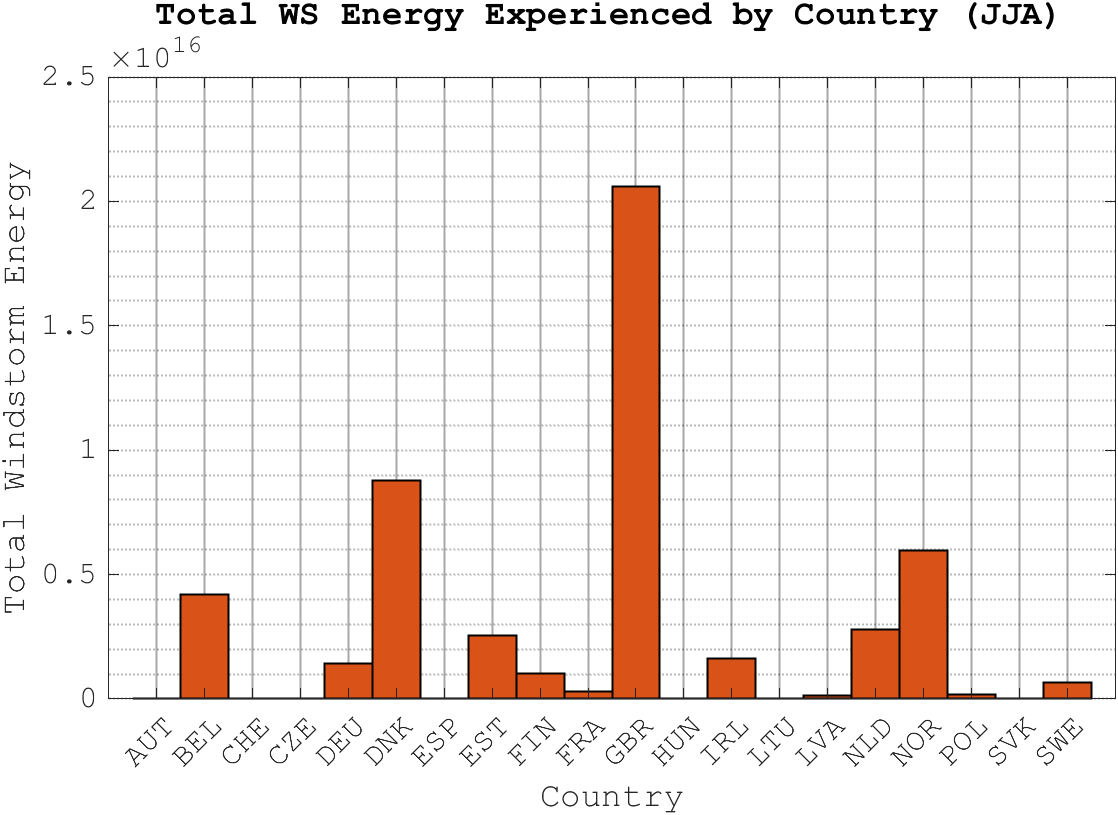
\includegraphics[width=\textwidth]{figures/Total Energy of WS JJA.png}
            \end{minipage}
            \hfill  % Fill horizontal space
            \begin{minipage}[t]{0.4\textwidth}
                \vspace*{-190pt}  % Move the start of the caption upwards. You might need to adjust this value.
                \caption{Represents the sum of WS energy recorded within the area of each country during Boreal Winter - December, January and February.}
                \label{fig:DJF_Tot_Eng_by_cunt}
                \vspace*{140pt}  % Increase space between captions. You might need to adjust this value.
                \caption{Represents the sum of WS energy recorded within the area of each country during Boreal Summer - June, July, August.}
                \label{fig:JJA_Tot_Eng_by_cunt}
            \end{minipage}
        \end{figure}
        %----------------------------------------------------------------------------------------------------------------------------------

    The second set of figures is presented in Figures \ref{fig:epcurvescountry}A-H. In them the exceedance probabilities of European countries along the east coast are presented. It begins from Spain in Figure \ref{fig:epcurvescountry}A, which is the southernmost country in the dataset of this study, and continues north. Along with the figure for each country, information is shown on the number of events that make up a curve. This is important when comparing the EP in a country versus the information in Figures \ref{fig:DJF_Tot_Eng_by_cunt} and \ref{fig:JJA_Tot_Eng_by_cunt} and Figures \ref{fig:naopostitivemap}, \ref{fig:naoneutralmapo} and \ref{fig:naonegativemapenter-label}. 

        % FIGURE 9 + 10 + 11 --------------------------------------------------------------------------------------------------------------
        \begin{figure}
            \centering
            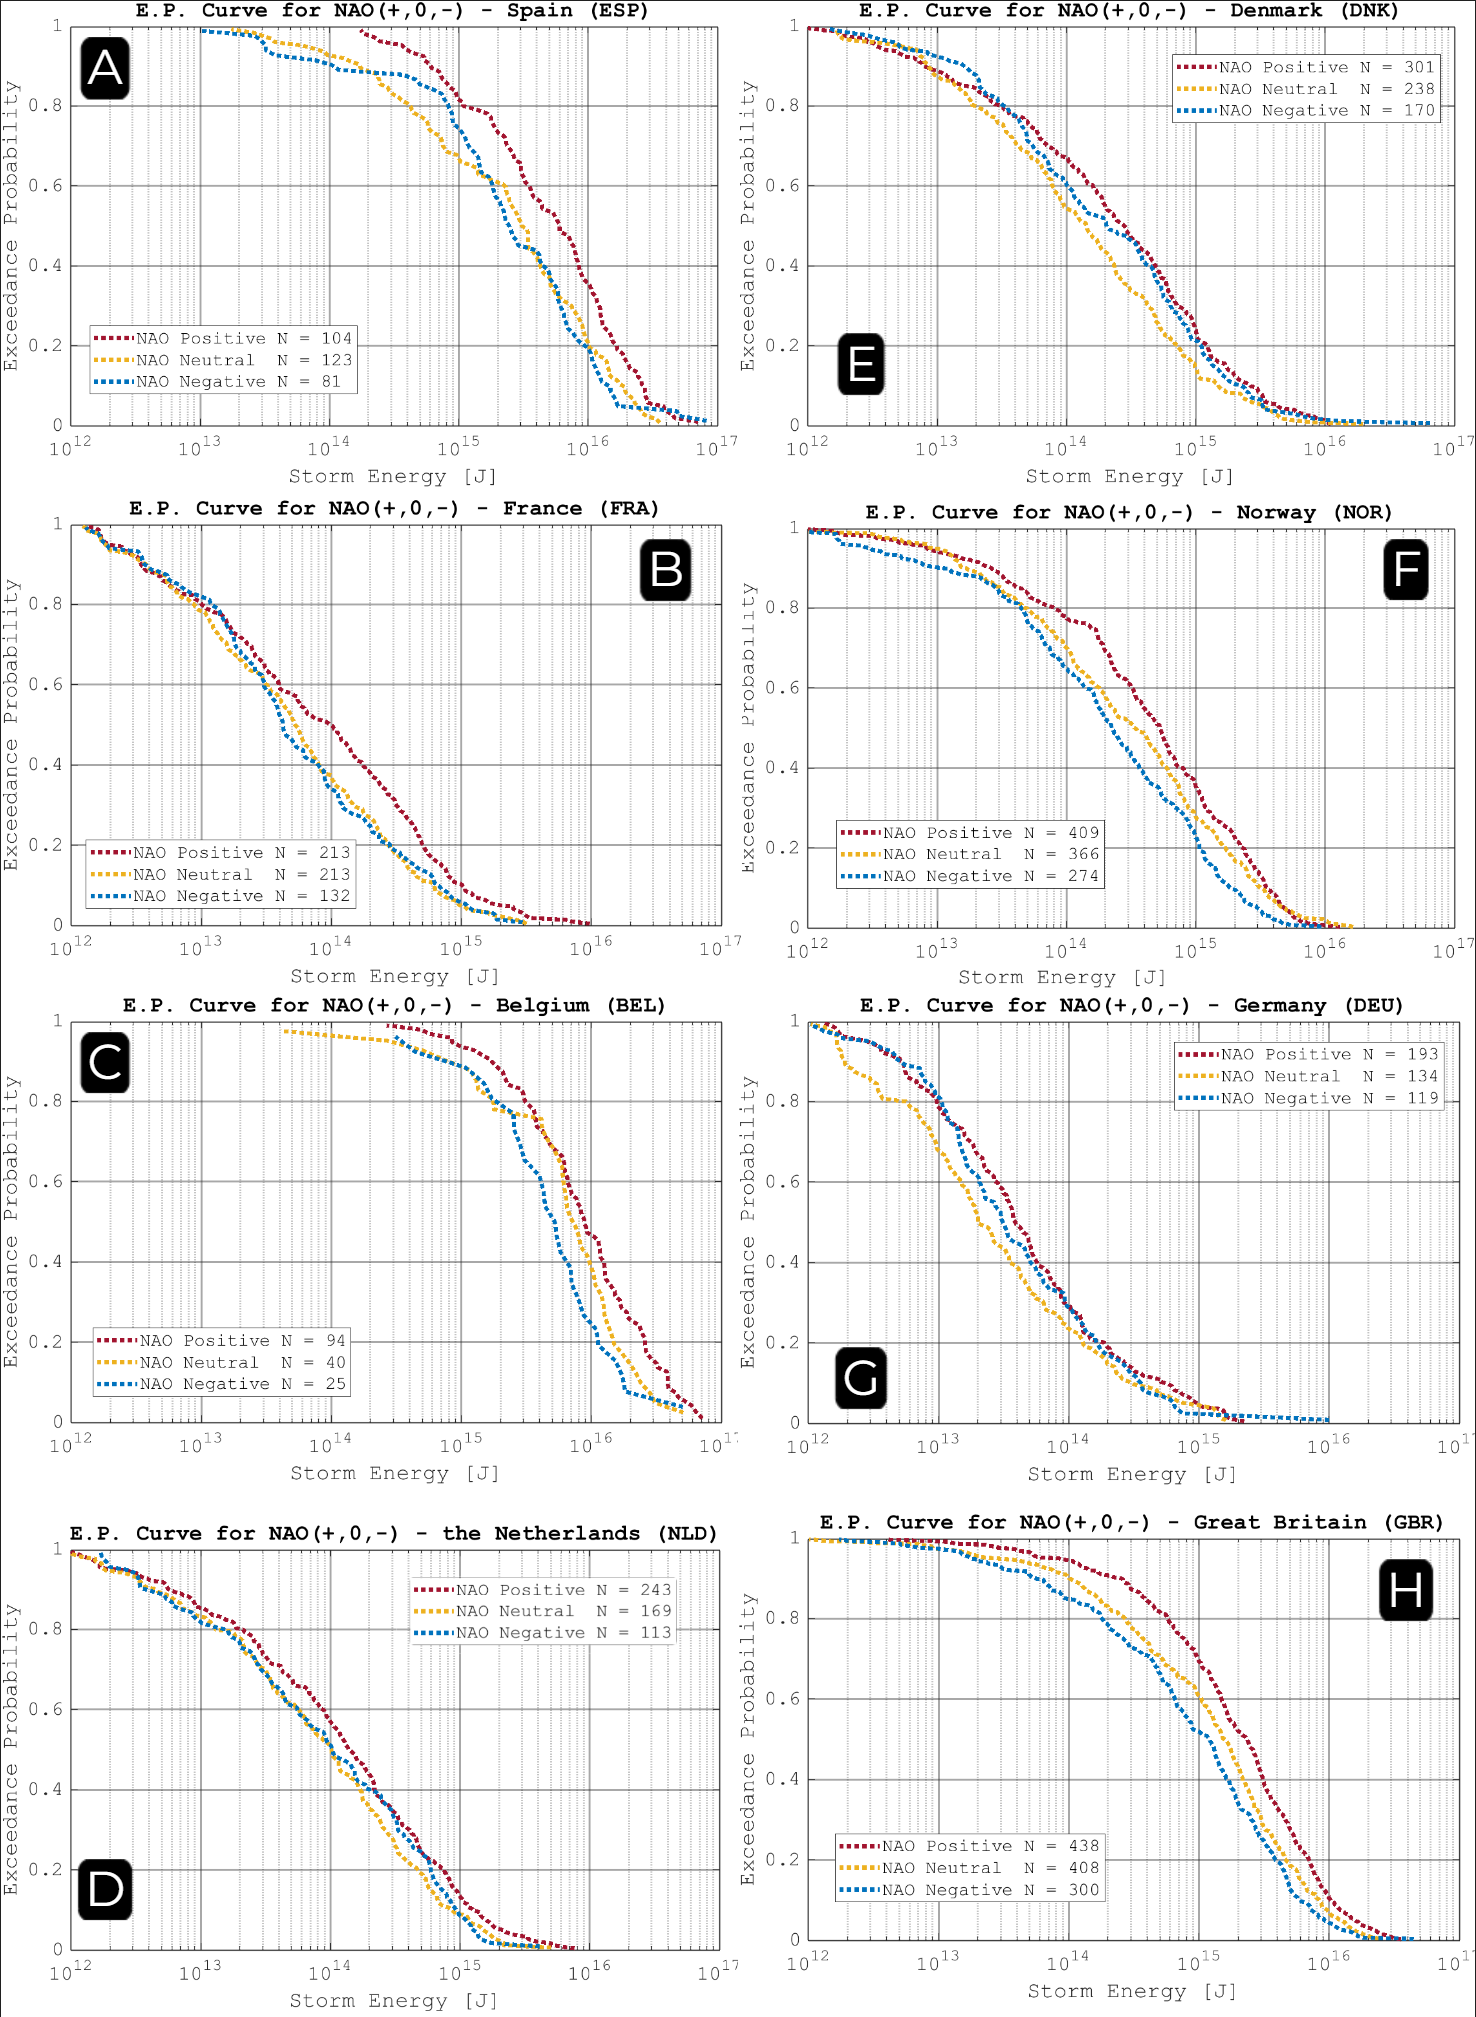
\includegraphics[width=\textwidth]{figures/epcurvescountry.png}
            \caption{Exceedance Probability for countries at the Western European border.}
            \label{fig:epcurvescountry}
        \end{figure}
        %----------------------------------------------------------------------------------------------------------------------------------
    







    
    
    


